\section{The Ballistic Pendulum}

\makelabheader %(Space for student name, etc., defined in master.tex or labmanual_formatting_commands.tex)

\textbf{Objectives} 

\begin{itemize}
\item To use a ballistic pendulum to determine the initial velocity of a projectile.
\item To apply the principles of conservation of momentum and mechanical energy to analyze a collision and subsequent motion.
\end{itemize}
\textbf{Overview }

In this lab, we will investigate the principles of momentum and energy conservation by using a ballistic pendulum to study collisions between a projectile and a target. A ballistic pendulum is a device that allows the measurement of a projectile's momentum by capturing it in a pendulum bob and observing the subsequent motion. This approach was historically significant in the study of ballistics and provided one of the first practical ways to measure the speed of bullets before the invention of high-speed chronographs.

Early researchers, including Benjamin Robins in the 18th century, developed the ballistic pendulum as a means to quantify the velocity of cannonballs and bullets. At the time, direct observation of fast-moving projectiles was impossible, so indirect measurements using pendulum motion were necessary. The device exploits the predictable relationship between the projectile's momentum and the motion of the pendulum to allow calculations of the projectile's speed.

In this experiment, we will launch a projectile into the pendulum and measure the resulting swing of the pendulum bob. Using the principles of conservation of momentum during the collision and conservation of energy during the pendulum's swing, we will calculate the initial speed of the projectile. Through this process, we will gain hands-on experience applying fundamental concepts of momentum, impulse, and energy in a real-world setting.

\textbf{Apparatus} 

\begin{itemize}
\item Ballistic pendulum
\item Carbon paper
\item C-Clamp, Large
\item Digital scale
\item Meter stick
\item Ruler
\item Ramrod
\item Safety goggles
\item Steel ball (25 mm diameter)
\end{itemize}

\textbf{Activity 0: Initial Measurements} 

(a) Detach the ballistic pendulum from the upright by unscrewing the top axle from the yoke. 

(b) Measure the mass $m_b$ of the steel ball and the mass $m_p$ of the pendulum and record them in the space below:
\vspace{5mm}

\hspace{0.5in}\( m_{b} =\) \hfill{}\( m_{p}= \) \hfill{}
\vspace{5mm}
\newpage	
(c) Measure the length $\ell$ of the pendulum arm. Make this measurement from the pivot point at the top of the pendulum to the center of mass of the ball/pendulum system. (See figure below.) 

\vspace{5mm}

\hspace{0.5in}\( \ell= \)
\answerspace{5mm}

(d) Reattach the ballistic pendulum to the upright. The long pin that extends from either side of the pendulum rod should be behind the angle indicator on the upright. Before continuing, have your instructor inspect the assembly.

\vspace{0.3cm}
{\par\centering 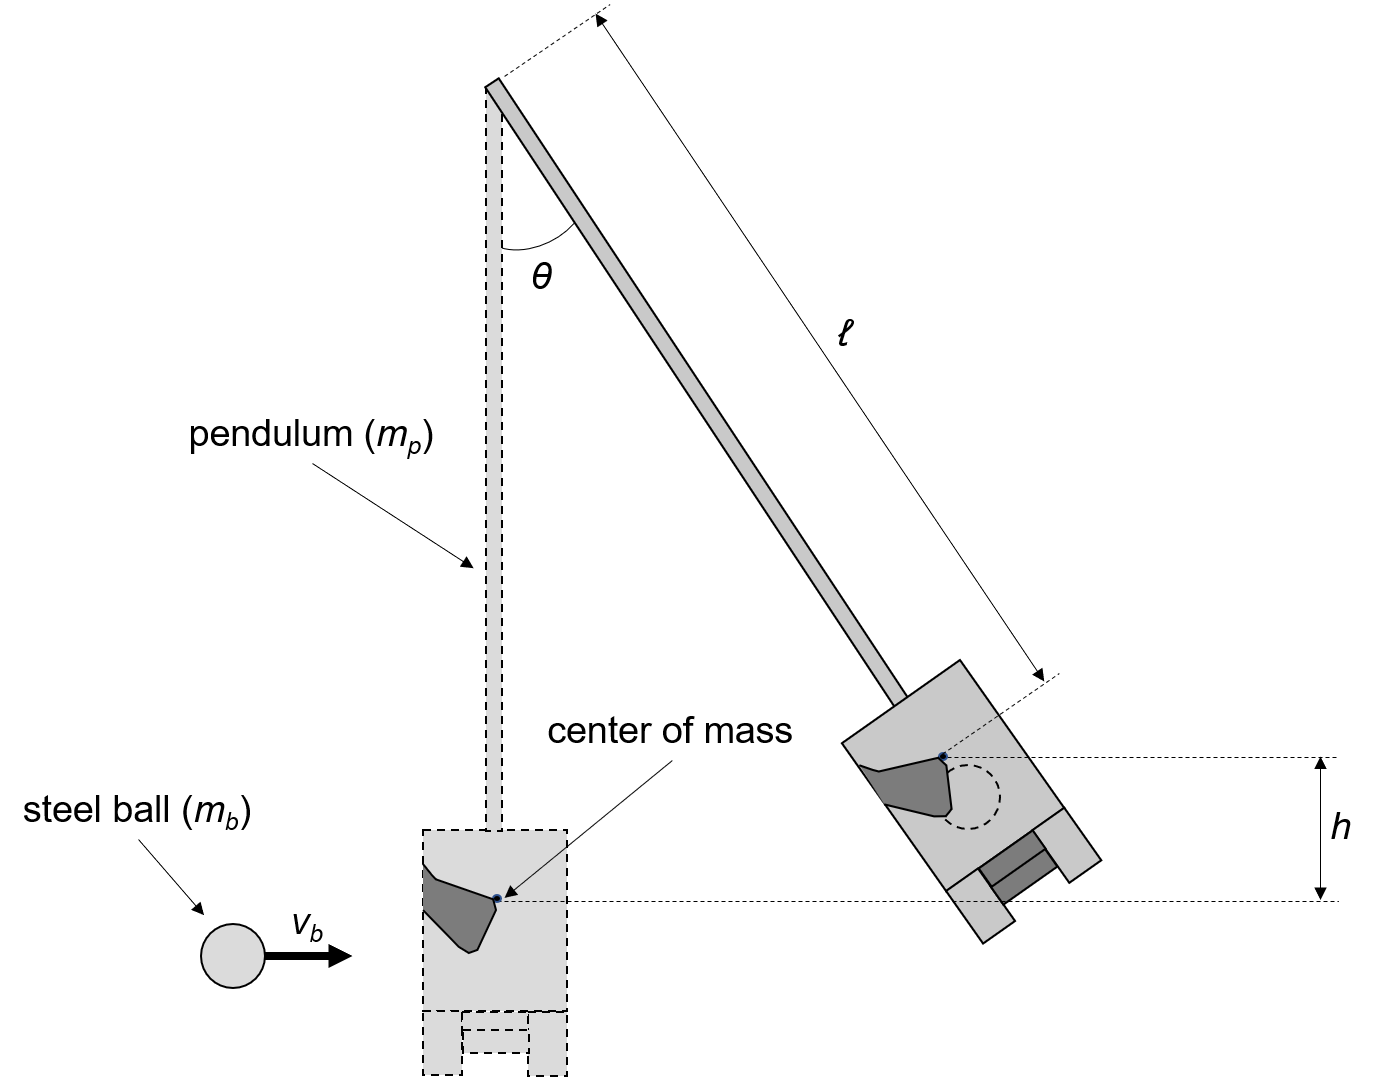
\includegraphics[height=3.5in]{ballistic_pendulum/ballistic_pendulum.png} \par}
\vspace{0.3cm}


\textbf{Activity 1: Theoretical Calculations}

(a) In the figure above, a ball collides with, and sticks to, a pendulum. How does the kinetic energy of the ball just before the collision compare to the kinetic energy of the combined ball-pendulum system immediately after the collision?
\answerspace{20mm}

(b) How does the momentum of the ball just before the collision compare to the momentum of the combined ball-pendulum system immediately after the collision? 
\answerspace{20mm}

(c) Note that the ball and pendulum stick together, making this an inelastic collision. In such collisions, momentum is conserved, but kinetic energy is not. Therefore, the kinetic energy of the system after the collision will be less than that of the incoming ball. If your reasoning in (a) or (b) led you to a different conclusion, please check your work or consult your instructor before continuing. 

(d) In this experiment, we will assume that the ball and the pendulum together act as a point mass located at their combined center of mass. Using conservation of momentum, write an equation for the speed $v_b$ of the ball just before the collision in terms of $m_b$, $m_p$, and $v_p$, where $v_p$ is the speed of the combined ball-pendulum immediately after the collision.
\answerspace{20mm}

(e) After the collision, the ball-pendulum combination swings upward to a maximum height $h$ relative to its starting point. Using conservation of mechanical energy, write an equation relating the speed $v_p$ of the ball-pendulum just after the collision to the height $h$ it rises.
\answerspace{20mm}

(f) It is often easier to measure the angle $\theta$ that the pendulum obtains at the peak of its swing rather than directly measuring the maximum height $h$. Write an equation relating the height $h$ to the angle $\theta$ and the pendulum length $\ell$.
\answerspace{20mm}

(g) Using the expressions obtained in parts (e) and (f), write an equation for $v_p$ in terms of $\theta$ and $\ell$.
\answerspace{20mm}

(h) Using the expressions obtained in parts (d) and (g), write an equation for the speed of the incoming ball $v_b$ in terms of $m_b$, $m_p$, $\theta$, and $\ell$.
\answerspace{20mm}

\textbf{Activity 2: The Experiment}

(a) Before proceeding, please put on your safety goggles.

(b) Load the steel ball into the launcher assembly. Use the ramrod to push the ball back as far as it will go. You should hear three ``clicks'' and the yellow band should be on the ``Long Range'' setting.

(c) Before firing the ball, make sure that the angle indicator on the upright is at $0^\circ$.

(d) Fire the ball. To do so, pull straight up on the trigger string.

(e) Observe the collision that occurs between the ball and the pendulum. Afterwards, use
the angle indicator to carefully measure and record the maximum angle, $\theta$, of the
ball-pendulum system. 

(f) Repeat the above experiment for a total of five trials. Make sure the pendulum is reset to $0^\circ$ each time.

(g) For each trial, calculate the speed $v_p$ of the ball-pendulum system immediately after the collision and the speed $v_b$ of the ball just before the collision.

\begin{center}
{\renewcommand{\arraystretch}{2.0}
\begin{tabular}{|c|c|C{0.8in}|C{0.8in}|} \hline 
$\theta$ (deg) & $h$ (m) & $v_p$ (m/s) & $v_b$ (m/s) \\ 
\hhline{|=|=|=|=|}
& & & \\ \hline 
& & & \\ \hline 
& & & \\ \hline 
& & & \\ \hline 
& & & \\ \hline  
\end{tabular} }
\end{center}
    
(h) Using your data for $v_b$, calculate the mean and standard deviation of the measured launch speed. Record your results below.
\answerspace{15mm}

\textbf{Activity 3: Testing Your Results}

In this activity, you will test your calculated launch speed by predicting and measuring where the projectile will land when fired horizontally from a lab table.

(a) Using your kinematic equations, derive an expression for the horizontal range $R$ of the ball when it is fired horizontally from the launcher a distance $H$ above the floor. Show all steps clearly.

1. Write an equation for the time of flight $t$ in terms of $H$ and $g$.
\answerspace{20mm}

2. Write an equation for the horizontal range $R$ in terms of $v_b$ and $t$.
\answerspace{20mm}

3. Combine your results to obtain $R$ in terms of $v_b$, $H$, and $g$.
\answerspace{20mm}
\newpage
(b) Move the launcher assembly to the edge of your lab table. Measure and record the vertical distance $H$ from the bottom of the launcher barrel to the floor.

\vspace{5mm}

\hspace{0.5in}\( H = \)
\answerspace{5mm}

(c) Using the average launch speed $\overline{v}_b$ obtained in Activity 2 and your measured value of $H$, calculate the predicted range of the projectile when fired horizontally.
\answerspace{35mm}

(d) Estimate the uncertainty in your predicted range, assuming that all of the uncertainty arises from the uncertainty in $v_b$.  
\answerspace{25mm}

(e) Tape a large sheet of paper to the floor at the predicted impact location. Place a sheet of carbon paper (carbon side down) on top so the projectile will leave a visible mark on impact.

(f) On the target paper, clearly mark the predicted range and the limits corresponding to your calculated uncertainty.

(g) Fire the projectile horizontally from the table and observe where it strikes the target paper. Measure and record the actual distance from the table edge to the impact point.

\begin{center}
{\renewcommand{\arraystretch}{2.0}
\begin{tabular}{|C{0.5in}|c|}
\hline
\textbf{Trial \#} & \textbf{Measured Range (m)} \\
\hhline{|=|=|}
1 & \\
\hline
2 & \\
\hline
3 & \\
\hline
4 & \\
\hline
5 & \\
\hline
\end{tabular}}
\end{center}

(h) Repeat the firing for a total of five trials, recording each impact position. Determine the mean and standard deviation of your measured ranges.
\answerspace{25mm}

(i) Compare your experimental results with your predicted range. Does your measured value fall within your calculated uncertainty? Briefly discuss possible sources of error or deviation.
\answerspace{25mm}
